\section{Induced Relational GCN}
\label{sec:gcn}
Now, we will encode the two label assignment mechanisms within a clique via a graph convolution. First, we briefly review Graph Convolution Networks (GCN) and identify some key concepts. Then, given the views $G_i$ for the four strategies, we show how to introduce label contrasts in~\Cref{subsec:contrast} followed by label sharing in~\Cref{subsec:similar}.

\subsection{Graph Convolution}
\label{subsec:graph}
Graph Convolution models adapt the convolution operations on regular grids (like images) to irregular graph-structured data $G = (V,E)$, learning low-dimensional vertex representations. If for example, we associate a scalar with each vertex $v \in V$, where $|V| = N$, then we can describe the convolution operation on a graph by the product of signal $x \in \mathbb{R}^N$ (feature vectors) with a learned filter $g_\theta$ in the fourier domain. Thus,
\begin{equation}
  g_\theta \ast x =  U \, g_\theta \, U^T x,
  \label{eq:basic_gcn}
\end{equation}
where, $\Lambda$ and $U$ are the eigenvalues and eigenvector of the normalized graph Laplacian, $L = I_N - D^{-\sfrac{1}{2}}AD^{\sfrac{1}{2}}$, and where $L = U \Lambda U^T$. $A$ denotes the adjacency matrix of a graph $G$ (associated with a view) with $N$ vertices. ~\Cref{eq:basic_gcn} implies a filter $g_\theta$ with $N$ free parameters, and requires expensive eigenvector decomposition of the adjacency matrix $A$. ~\citet{deferrard} proposed to approximate $g_\theta$, which in general is a function of $\Lambda$, by a sum of Chebyshev polynomials $T_k(x)$ up to the $k$-th order. Then,

\begin{equation}
  g_\theta \ast x \approx U \, \sum_{k=0}^K \theta_k T_k(\tilde{\Lambda}) \, U^T x \approx \, \sum_{k=0}^K \theta_k T_k(\tilde{L}) \, x,
  \label{eq:approx_gcn}
\end{equation}
where, $\tilde{\Lambda} = 2 \Lambda/ \lambda_{\max}- I_N$ are the scaled eigenvalues and $\tilde{L} = 2L/\lambda_{max} - I_N$ is the corresponding scaled Laplacian. Since $\tilde{L} = U \tilde{\Lambda} U^T$, the two equations are approximately equal.

The key result from~\citet{deferrard} is that~\Cref{eq:approx_gcn} implies $k$-hop localization---the convolution result depends only on the $k$-hop neighborhood. In other words,~\Cref{eq:approx_gcn}  is a $k$-hop approximation.

However, since we use equivalence relations in our framework that result in cliques, we can do an \textit{exact} convolution operation since vertices in a clique only have one-hop (i.e., $k=1$) neighbors (see lemma 5.2, \cite{Hammond2011}). The resulting convolution is linear in $L$ and now has only two filter parameters, $\theta_{0}$ and $\theta_{1}$ shared over the whole graph.
\begin{equation}
g_{\theta} * x = \theta_{0}x + \theta_{1}\left(L-I_{N} \right)x %\\
\label{eq:restrictk}
\end{equation}

We emphasize the distinction with~\citet{gcn} who approximate the~\citet{deferrard} observation by restricting $k=1$. They do so since they work on arbitrary graphs; since our relations result in views with cliques, we do not make any approximation by using $k=1$.

\begin{figure}[h]
  \centering
  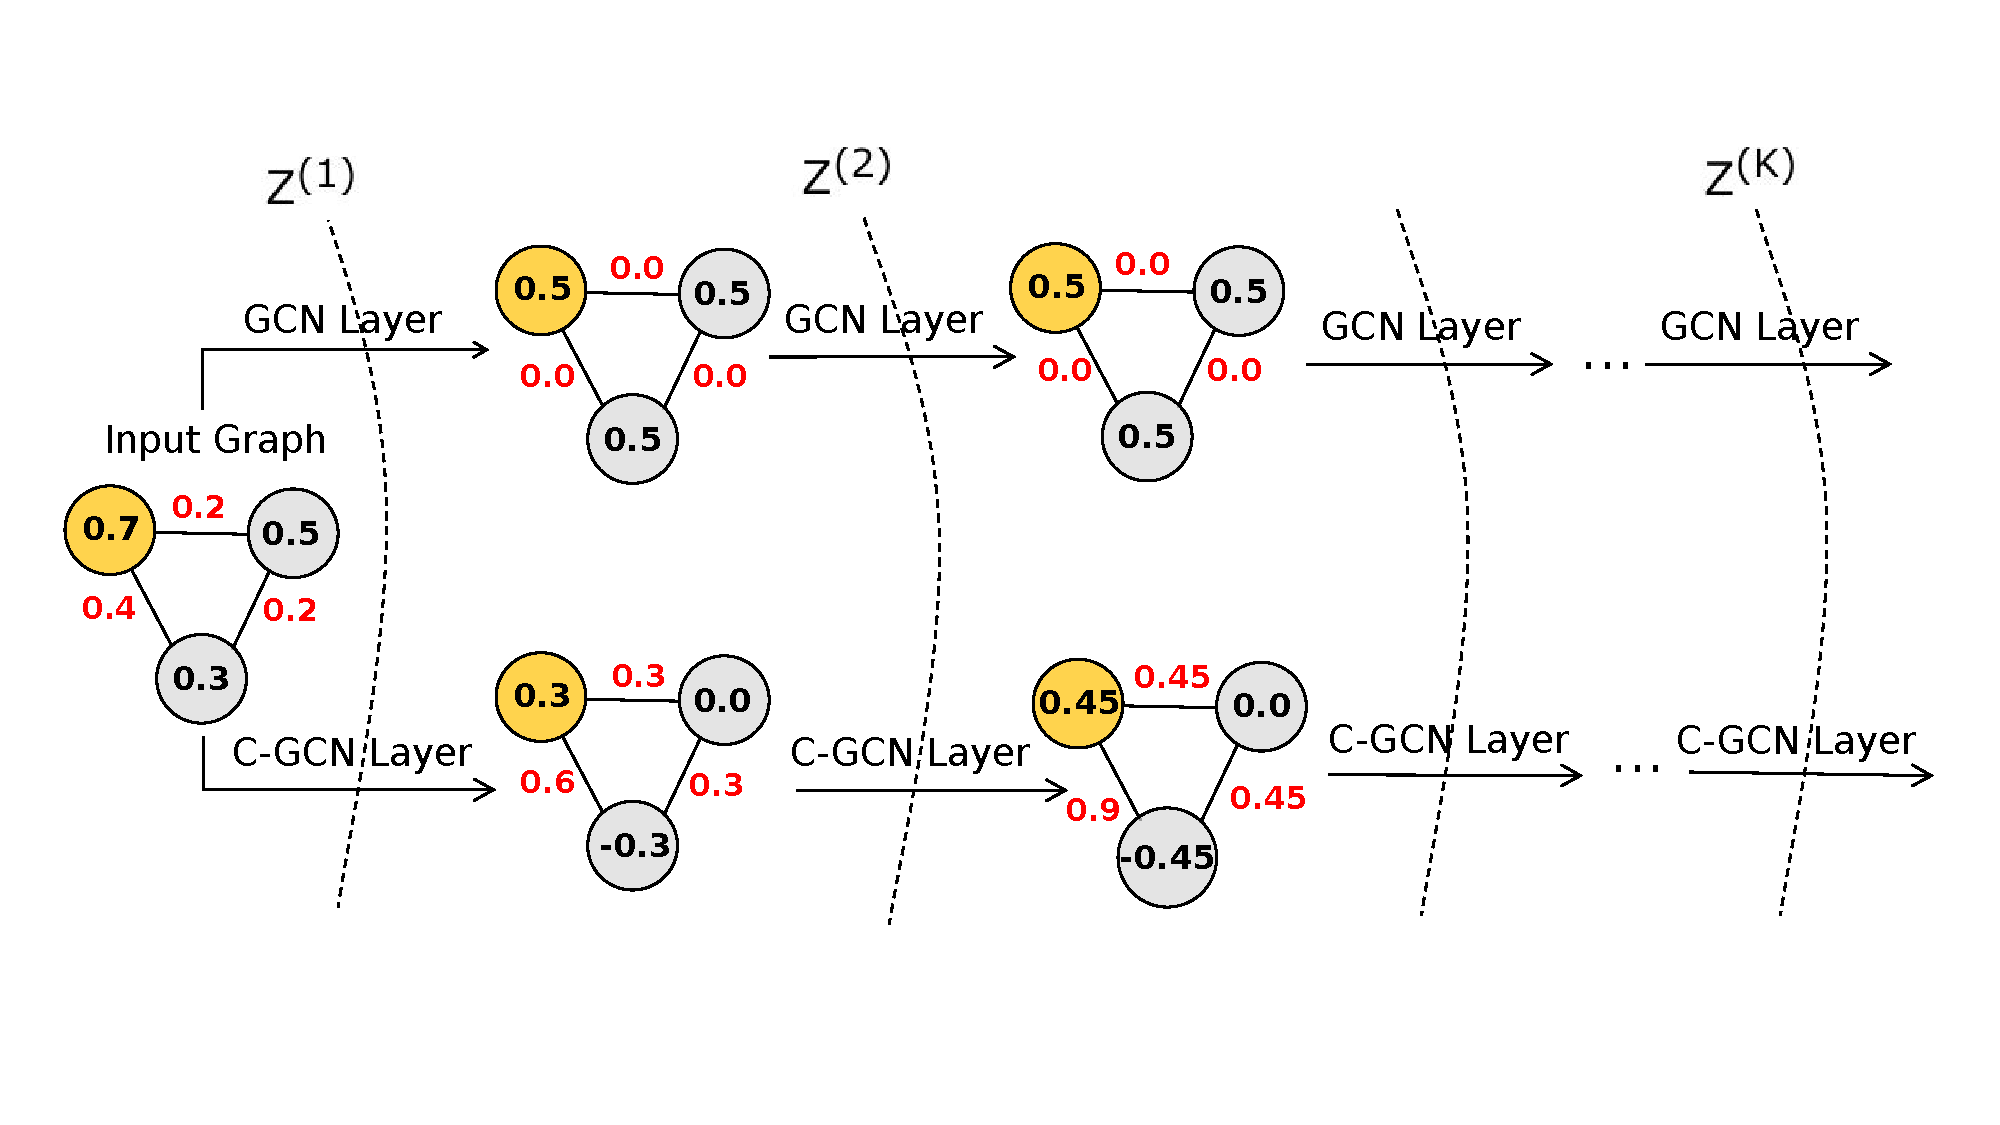
\includegraphics[scale=0.43]{figures/fig_contrast}
  \caption{\label{fig:contrast}Stylized example showing the convolution results of GCN and proposed Contrastive GCN for a question with three answers. Edge labels denote the feature difference while node labels denote the resulting feature value. The feature difference between neighboring nodes increases with each convolution layer for Contrastive GCN while GCN averages the feature values among nodes. }
\end{figure}

\subsection{Contrastive Graph Convolution}
\label{subsec:contrast}
Now, we show how to perform graph convolution to encode the mechanism of contrast, where label assignments for a tuple depend on the contrast with its neighborhood.

To establish contrast, we need to compute the \emph{difference} between the vertex's own features to its neighborhood in the clique. Thus we transform~\Cref{eq:restrictk} by setting $\theta = \theta_{0}$ = $\theta_{1}$, which essentially restricts the filters learned by the GCN. This transformation leads to the following convolution operation:
\begin{align}
g_{\theta} * x & =  \theta \left( I_N + L- I_{N} \right) x \\
g_{\theta} * x & =  \theta \left( I_N - D^{-\sfrac{1}{2}} A D^{-\sfrac{1}{2}}\right) x \label{eq:contrastdetail}
\end{align}

Notice that~\Cref{eq:contrastdetail} says that for example, for any vertex $u$ with a scalar feature value $x_u$, for a given clique with $n \geq 2$ vertices, the convolution operation computes a new value $\hat{x}_u$ for vertex $u$ as follows:
\begin{equation}
  \hat{x}_u = \theta \left ( x_u - \frac{1}{n-1} \sum_{v \in \mathcal{N}_u} x_v \right ).
\end{equation}
where $\mathcal{N}_u$ is the neighborhood of vertex $u$. Notice that since our equivalence relations construct cliques, for all vertices $u$ that belong to a clique of size $n$, $|\mathcal{N}_u| = n-1$.

When we apply the convolution operation in~\Cref{eq:contrastdetail} at each layer of GCN, output for the $k$-th layer is:

\begin{equation}
  \label{eq:contrast}
  \mathbf{Z}_c^{k} = \sigma \left( \left (I_N - D^{-\sfrac{1}{2}}A_cD^{\sfrac{1}{2}} \right) \mathbf{Z}_c^{k-1} \mathbf{W}_c^{k}\right)
\end{equation}
with $A_c$ denoting the adjacency matrix in the contrastive view. $\mathbf{Z}_c^{k} \in \mathbb{R}^{N \times d}$ are the learned vertex representations for each $(q,a)$ tuple under the contrastive label assignment. $N$ is the total number of tuples and $d$ refers to the dimensionality of the embedding space. $\mathbf{Z}^{k-1}$ refers to the output of the previous $(k-1)$-{th} layer, and $\mathbf{Z}^{0} = X$ where $X$ is the input feature matrix. $\mathbf{W}_c^{k}$ are the filter $\theta$ parameters learnt by the GCN; $\sigma( \cdot)$ denotes the activation function (e.g. ReLU, $\tanh$).

To understand the effect of~\Cref{eq:contrast} on a tuple, let us restrict our attention to a vertex $u$ in a clique of size $n$. We can do this since the convolution result in one clique is unaffected by other cliques. When we do this, we obtain:
\begin{equation}
  z_c^{k}(u) = \sigma \left(\left(z_c^{k-1}(u) - \frac{1}{n-1} \sum_{v \in \mathcal{N}_u} z_c^{k-1}(v) \right) \mathbf{W}_{c}^{k}\right). \label{eq:contrastrestrict}
  \end{equation}

Now consider a pair of contrasting vertices, $u$ and $v$ in the same clique of size $n$. Let us ignore the linear transform by setting $W_{c}^{k}=\mathbf{I}$ and set $\sigma(\cdot)$ to the identity function. Then we can easily verify that:
\begin{equation}
z_c^{k}(u) - z_c^{k}(v) = \underbrace{
  \left (1 + \frac{1}{n-1} \right )
  }_{\text{magnification}}
  \times
  \underbrace{
    \left ( z_c^{k-1}(u) - z_c^{k-1}(v) \right )
    }_{\text{contrast in previous layer}}, \label{eq:disccontrastsimple}
\end{equation}
where, $z_c^{k}(u)$ denotes the output of the $k$-th convolution layer for the $u$-th vertex in the contrastive view. As a result, each convolutional layer magnifies the feature contrast between the vertices that belong to the same clique. Thus, the contrasting vertices move further apart. We term this as \emph{Discriminative Feature Magnification} and~\Cref{eq:disccontrastsimple} implies that we should see higher magnification effect for smaller cliques.
An illustration is provided in the bottom part of the \cref{fig:contrast} with a uni-dimensional feature.

Contrasting nodes are shifted further apart by \cref{eq:contrast} improving their separability in the learned manifold (further discussion in \cref{ref:analysis}).

\subsection{Encoding Similarity Convolution}
\label{subsec:similar}
We next discuss how to encode the mechanism of sharing labels in a GCN. While label sharing applies to our similar contrast relation (two strategies: Arrival similarity; TrueSkill similarity, see~\Cref{sub:Induced Views}), it is also trivially applicable to the reflexive relation, where the label of the tuple only depends on itself. First, we discuss the case of similar contrasts.

\noindent
\textbf{Encoding Similar Contrasts:}
\label{sub:Encoding Similar Contrasts}
To encode label sharing for the two similar by contrast cases, we transform~\Cref{eq:restrictk} with the assumption $\theta = \theta_0 = -\theta_1$. Thus

\begin{equation}
g_{\theta} * x = \theta\left(I_{N} + D^{-\sfrac{1}{2}}AD^{-\sfrac{1}{2}}\right) x, \label{eq:similargcn}
\end{equation}

Similar to the ~\Cref{eq:contrastdetail} analysis, convolution operation in \Cref{eq:similargcn} computes a new value $\hat{x}_u$ for vertex $u$ as follows:
\begin{align}
  \hat{x}_u &= \theta \left ( x_u + \frac{1}{n-1} \sum_{v \in \mathcal{N}_u} x_v \right ).\\
  \hat{x}_u &= \theta \left ( \frac{n-2}{n-1} x_u + \frac{n}{n-1} \mu_x \right ).
\end{align}
That is, in the mechanism where we share labels in a clique, the convolution pushes the values of each vertex in the clique to the average feature value, $\mu_x = \frac{1}{n} \sum_{v \in \mathcal{N}_u \cup u} x_v$, in the clique.

When we apply the convolution operation in~\Cref{eq:similargcn} at each layer of GCN, output for the $k$-th layer:
\begin{equation}
  \label{eq:similar}
  \mathbf{Z}_s^{k} = \sigma \left( \left (I_N + D^{-\sfrac{1}{2}}A_sD^{\sfrac{1}{2}} \right) \mathbf{Z}_s^{k-1} \mathbf{W}_s^{k}\right)
\end{equation}
with $A_s$ denoting the adjacency matrix in the similar views.

We analyze the similarity GCN in a maner akin to~\Cref{eq:contrastrestrict} and we can easily verify that:

\begin{equation}
z_s^{k}(u) - z_s^{k}(v) = \underbrace{
  \left (1 - \frac{1}{n-1} \right )
  }_{\text{reduction}}
  \times
  \underbrace{
    \left ( z_s^{k-1}(u) - z_s^{k-1}(v) \right )
    }_{\text{contrast in previous layer}}, \label{eq:diffsimilar}
\end{equation}
where, $z_s^{k}(i)$ denotes the output of the $k$-th convolution layer for the $i$-th vertex in the similar view. As a result, each convolutional layer reduces the feature contrast between the vertices that belong to the same clique. Thus, the similar vertices move closer (see top part in ~\cref{fig:contrast}).

The proposed label sharing encoding applies to both similar contrast strategies (TrueSkill; Arrival). We refer to the corresponding vertex representations as $\mathbf{Z}_{ts}^{k}$ (TrueSkill), $\mathbf{Z}_{as}^{k}$ (Arrival).

\noindent
\textbf{Reflexive Convolution:}
\label{subsubsec:reflex}
We encode the reflexive relation with self-loops in the graph resulting in an identity adjacency matrix. This relation is the trivial label sharing case, with an independent assignment of vertex labels. Thus, the output of the $k$-th convolutional layer for the reflexive view, $\mathbf{Z}_r^{k}$ reduces to:
\begin{equation}
  \label{eq:reflexive}
  \mathbf{Z}_r^{k} = \sigma \left( I_N \mathbf{Z}_r^{k-1} \mathbf{W}_r^{k} \right)
\end{equation}
Hence, the reflexive convolution operation is equivalent to a feedforward neural network with multiple layers and activation $\sigma( \cdot )$.

\vspace{0.1in}
\noindent
Each strategy $S_i \in \mathbf{S}$ belongs to one of the three relation types---reflexive, contrastive and similarity, where $\mathbf{R}$ denotes the set of strategies of that relation type. $\mathcal{R} = \bigcup \mathbf{R}$ denotes the set of all relation types.
$\mathbf{Z}_i^K \in \mathbb{R}^{N X d}$ represents the $d$ dimensional vertex embeddings for strategy $S_i$ at the $K$-th layer. For each strategy $S_i$, we obtain a scalar score by multiplying $\mathbf{Z}_i^K$ with transform parameters $\widetilde{W}_i \in \mathbb{R}^{d \times 1}$.
The sum of these scores gives the combined prediction score, $\mathbf{H}_{\mathbf{R}} \in \mathbb{R}^{N X 1}$, for that relation type.
\begin{equation}
    \label{eq:score}
        \mathbf{H}_{\mathbf{R}} = \sum_{S_i \in \mathbf{R}} \mathbf{Z}_i^K \widetilde{W}_i^T
\end{equation}

In this section, we proposed Graph Convolutional architectures to compute vertex representations of each $(q,a)$ tuple under the four strategies.
In particular, we showed how to encode two different label assignment mechanisms---label sharing and determine label based on contrast---within a clique. The architecture that encodes label assignment based on contrast is a novel contribution; distinct from the formulations presented by~\citet{gcn} and its extensions~\cite{signedgcn, relationalGCN}. Prior convolutional architectures implicitly encode the label sharing mechanism (~\cref{eq:similargcn}); however, label sharing is unsuitable for contrastive relationships across vertices. Hence our architecture fills this gap in prior work.
